\section{Quantum Modular Multiplication}
\label{sec:csa-mod-mult}

We can build upon our carry-save adder to implement quantum modular
multiplication in logarithmic depth. We start with a completely classical
problem to illustrate the principle of multiplication by repeated addition.
Then we consider modular multiplication of two quantum integers in a serial
and a parallel fashion in Section
\ref{subsec:csa-mod-mult-qq}. Both of these problems use as subroutines
\emph{partial product creation}, which we define and solve
 in Section \ref{subsec:ppc} and
 \emph{modular multiple addition}, which we define and solve
in Section \ref{subsec:mma}.

%%%%%%%%%%%%%%%%%%%%%%%%%%%%%%%%%%%%%%%%%%%%%%%%%%%%%%%%%%%%%%%%%%%%%%%%%%%%%%%
First we consider a completely classical problem:
given three $n$-bit classical numbers $a$, $b$, and $m$,
compute $c = ab \bmod m$, where $c$ is allowed to be in CSE.

We only have to add shifted
multiples of $a$ to itself, ``controlled'' on the bits of $b$. There are
$n$ shifted multiples of $a$, let's call them $z^{(i)}$, one for every bit of $b$:
%%\begin{equation}
$z^{(i)} = 2^i a b_i \bmod m$.
%%\end{equation}
We can parallelize the addition of $n$ numbers in a logarithmic depth
binary tree to get a total depth of $O(\log n)$.

%%%%%%%%%%%%%%%%%%%%%%%%%%%%%%%%%%%%%%%%%%%%%%%%%%%%%%%%%%%%%%%%%%%%%%%%%%%%%%
\subsection{Modular Multiplication of Two Quantum Integers}
\label{subsec:csa-mod-mult-qq}

We now consider the problem of multiplying a classical number controlled
on a quantum bit with a
\emph{quantum integer},
which is a
quantum superposition of classical numbers.\footnote{In this paper, an $n$-qubit 
quantum integer is a
general superposition of up to $2^n$ classical integers. As a special case,
a classical number controlled on a single qubit is a superposition of
$2$ classical integers. This should not be confused with quantum numbers
in physics.}

\begin{quote}
Given an $n$-qubit quantum integer $\ket{x}$, a control qubit $\ket{p}$,
and two $n$-bit classical numbers $a$
and $m$,
compute $\ket{c} = \ket{xa[m]}$, where $c$ is allowed to be in CSE.
\end{quote}

This problem occurs naturally in modular exponentiation (described in
the next section) and can be considered \emph{serial multiplication},
in that $t$ quantum integers are multiplied in series to a single
quantum register. This is used in serial QPF as mentioned in
Section \ref{sec:fpl-related}.


We first create $n$ quantum integers $\ket{z^{(i)}}$,
which are shifted multiples of the classical number $a$ controlled on the bits
of $x$:
\begin{equation}
\ket{z^{(i)}} \equiv \ket{2^i a[m] \cdot x_i }.
\end{equation}
These are typically called \emph{partial products} in a classical multiplier.
How do we create these numbers, and what is the depth of the procedure?
First, note that $\ket{2^i a[m]}$ is a classical number, so we can
precompute them classically and prepare them in parallel using single-qubit
operations
on $n$ registers, each consisting of $n$ ancillae qubits. Each $n$-qubit
register will hold a future $\ket{z^{(i)}}$ value.
We then fan out each of the
$n$ bits of $x$, $n$ times each, using an unbounded fanout operation so that
$n$ copies of each bit $\ket{x_i}$ are next to register $\ket{z^{(i)}}$.
This takes a total of $O(n^2)$ parallel CNOT operations.
We then entangle each $\ket{z^{(i)}}$ with the corresponding $x_i$.
%The schematic for this is shown in Figure \ref{fig:mod-mult-create}.
After this, we interleave these numbers into groups of three using
constant-depth teleportation. This reduces to the task of modular
multiple addition in order to add these numbers down to a single
(CSE) number modulo $m$, which is described in Section \ref{subsec:mma}.

%\begin{figure*}[htp!]
%\centerline{
%\includegraphics[width=4.5in]{./znumbers.pdf}
%}
%\caption{Creating $n=4$ shifted values $\{z^{(0)},z^{(1)},z^{(2)},z^{(3)}\}$
%for an input number $x$.}
%\label{fig:mod-mult-create}
%\end{figure*}

Finally, we tackle the most interesting problem:
\begin{quote}
Given two $n$-qubit quantum integers $\ket{x}$ and
$\ket{y}$ and an $n$-bit classical number
$m$,
compute $\ket{c} = \ket{xy \bmod m}$,
where $\ket{c}$ is allowed to be in CSE.
\end{quote}

This can be considered \emph{parallel multiplication} and is responsible
for our logarithmic speedup in modular exponentiation and parallel QPF.

Instead of creating $n$ quantum integers $\ket{z^{(i)}}$, we must create
up to $n^2$ numbers
$\ket{z^{i,j}}$ for all possible pairs of quantum bits $x_i$ and $y_j$,
$i,j \in \{0,\ldots,n-1\}$:
\begin{equation}
\ket{z^{i,j}} \equiv \ket{2^i2^j[m]\cdot x_i \cdot y_j}.
\label{eqn:zij-pp}
\end{equation}
We create these numbers using a similar procedure to the previous problem.
Adding $n^2$ quantum integers of $n$ qubits each takes depth
$O(\log(n^2))$, which is still $O(\log n)$.
Creating $n^2\times n$-bit quantum integers takes width $O(n^3)$.
Numerical constants are given for these resource estimates in
Section \ref{subsec:mod-mult-resources} for the entire modular multiplier.

Here is an outline of our modular multiplier construction, combining the
two halves of partial product creation (Section \ref{subsec:ppc}) and
modular multiple addition (Section \ref{subsec:mma}).
This is the first building block which requires multiple modules,
and hence the full generality of the \textsf{2D CCNTCM} model. 

\begin{enumerate}
\item Initially, the inputs consist of the CSE quantum integers $x$ and $y$,
each with $2n+3$ bits, sitting on adjacent edges of a square lattice that has
sides of length $3(2n+3)$ qubits.
\item For each of $\lceil \log_2 (2n+3) \rceil$ rounds:
\begin{enumerate}
\item Of the existing $\{x_i\}$ and $\{y_j\}$ bits, apply a CNOT to create an
entangled copy in an adjacent qubit.
\item Teleport this new copy halfway between its current location and the
new copy.
\item At every site where an $\ket{x_i}$ and an $\ket{y_j}$ meet,
apply a Toffoli gate to create $\ket{x_i \cdot y_j}$.
\item Teleport $\ket{x_i \cdot y_j}$ to the correct $z$-site module.
\end{enumerate}
\item Within each $z$-site module, fanout $\ket{x_i \cdot y_j}$ up to $n$
times, corresponding to each $1$ in the modular residue $2^i 2^j \bmod m$,
to create the $n$-qubit quantum integer $\ket{z^{(i,j)}}$.
\item For each triplet of $z$-site modules, teleport the quantum integers
$\ket{z^{(i,j)}}$ to a CSA tile module, interleaving the three numbers so that
bits of the same significance are adjacent. This concludes partial product
creation (Section \ref{subsec:ppc}).
\item Perform modular multiple addition (described in Section \ref{subsec:mma})
on $t'$ $n$-qubit quantum integers down to 2 $n$-qubit quantum integers (one CSE number).
\item Uncompute all the previous steps to restore ancillae to $\ket{0}$.
\end{enumerate}
%%%%%%%%%%%%%%%%%%%%%%%%%%%%%%%%%%%%%%%%%%%%%%%%%%%%%%%%%%%%%%%%%%%%%%%%%%%%%%%
\subsection{Partial Product Creation}
\label{subsec:ppc}

This subroutine describes the procedure of creating $t'=O(n^2)$ partial products of
the CSE quantum integers $x$ and $y$, each with $2n+3$ bits each. We will now
discuss only the case of parallel multiplication. Although we
will not provide an explicit circuit for this subroutine, we will outline
our particular construction and give a numerical upper bound on the
resources required.

First, we need to generate the product bits
$\ket{x_i\cdot y_j}$ for all possible $(2n+3)^2$ pairs of $\ket{x_i}$ and
$\ket{y_j}$.
A particular product bit $\ket{x_i \cdot y_j}$
controls a particular classical number, the
$n$-bit modular residue $2^i 2^j [m]$, to form the partial product
$\ket{z^{(i,j)}}$ defined in Equation \ref{eqn:zij-pp}.
However, some of these partial products
consist of only a single qubit, if $2^i 2^j < 2^n$, which is the minimum
value for an $n$-bit modulus $m$. There are at least $2n^2 - 2n + 1$
such single-bit partial products, which can be grouped into at most
$(2n+3)\times n$-bit numbers. Of the $(2n+3)^2$ possible partial products,
this leaves the number of remaining $n$-bit partial products as at most
$2n^2 + 14n +8$. Therefore we have a maximum number of $n$-bit
partial products, which we will simply refer to as $t'$ from now on.
% from N16, p. 65
\begin{equation}
t'=2n^2+16n+11
\label{eqn:tprime}
\end{equation}
%
The creation of the product bits $\ket{x_i \cdot y_j}$ occurs on a
square lattice of $(3(2n+3))^2$ qubits, with the numbers $\ket{x_i}$ and
$\ket{y_j}$ located on adjacent edges. The factor of $3$ in the size of the lattice
allows the $\ket{x_i}$ and $\ket{y_j}$ bits to teleport past each other.
The $\ket{x_i}$ bits are teleported along an axis that is perpendicular to
the teleportation axis for the $\ket{y_j}$ bits, and vice versa.
Product bit creation, and this square lattice, comprise a single module.
In $\lceil \log_2 (2n+3) \rceil$
rounds, these bits are copied via a CNOT and teleported to the middle of
a recursively halved interval of the grid. The copied bits $\ket{x_i}$ and
$\ket{y_j}$
first form $1$ line, then $3$ lines, then $7$ lines, and so forth,
intersecting at $1$ site, then $9$ sites, then $49$ sites, and so forth.
There are $\lceil \log_2 (2n+3) \rceil$ such rounds.

At each intersection, a Toffoli gate is used to create $\ket{x_i \cdot y_j}$
from the given $\ket{x_i}$ and $\ket{y_j}$. These product bits are then
teleported away from this qubit, out of this product bit module, to different
modules where the $\ket{z^{(i,j)}}$ numbers are later generated,
called $z$-sites. There are $t'$ $z$-site modules which each contain 
an $n$-qubit quantum integer. Any
round of partial product generation will produce at most as many product
bits $x_i \cdot y_j$ as in the last round, which is half the total number
of $(2n+3)^2$.
%These product bits are teleported out the two sides of the
%square lattice that are opposite the input numbers $x$ and $y$, which means the
%square lattice has dimension at most $((2(2n+3)-1)(n+2))^2 = O(n^4)$.

%The $z$-sites have total width of $3nt'$ qubits, so the maximum total
%teleportation length of all qubits is $(2n+3)^2$ multiplied by the maximum
%length of any single teleportation length,
%Our construction consists of the following steps:

We now present the resources for partial product creation, the first half of
a modular multiplier, including the reverse computation.

The circuit depth is $O(\log n)$:
%
\begin{equation}
D_{PPC} = 32\log_2 n + 150\text{.}
\end{equation}
%
The module depth is $O(1)$:
%
\begin{equation}
\overline{D}_{PPC} = 8\text{.}
\end{equation}
%
The circuit size is $O(n^3)$:
%
\begin{eqnarray}
S_{PPC} & = & (6n + 9)\log_2 n +\\
        &   & (26n^3 + 232n^2 + 224n + 159)\text{.}
\end{eqnarray}
%
The module size is $O(n^2)$:
%
\begin{eqnarray}
\overline{S}_{PPC} = 6n^2 + 26n + 19\text{.}
\end{eqnarray}
%
The circuit width is $O(n^3)$:
%
\begin{eqnarray}
W_{PPC} = 6n^3 + 48n^2 - 8n + 1\text{.}
\end{eqnarray}
%
The module width is $O(n^2)$:
% N18 p. 3
\begin{eqnarray}
\overline{W}_{PPC} = 2n^2 + 16n + 12\text{.}
\end{eqnarray}

%%%%%%%%%%%%%%%%%%%%%%%%%%%%%%%%%%%%%%%%%%%%%%%%%%%%%%%%%%%%%%%%%%%%%%%%%%%%%%%
\subsection{Modular Multiple Addition}
\label{subsec:mma}

As a subroutine to modular multiplication, we define the operation of
repeatedly adding multiple numbers down to a single CSE number, called
\emph{modular multiple addition}.

The modular multiple addition circuit generically adds down $t'\times n$-bit
conventional numbers to an $n$-bit CSE number:
%
\begin{equation}
z^{(1)} + z^{(2)} + \ldots z^{(t')} \equiv (u+v)[m].
\end{equation}
%
It does not matter how the
$t'$ numbers are generated, as long as they are divided into groups of three
and have their bits interleaved to be the inputs of a CSA tile.
From the previous section, serial multiplication results in
$t' \in O(n)$ and parallel multiplication results in $t' \in O(n^2)$. Each CSA tile
is contained in its own module. These modules are arranged in layers within
a logarithmic depth binary tree, where 
the first layer contains $\lceil t'/3 \rceil$ modules. A modular addition
occurs in all the modules of the first layer in parallel. The outputs from this
first layer are then teleported to be the inputs of the next layer of modules,
which have at most two-thirds as many modules. This continues until the
tree terminates in a single module, whose output is a CSE number $u+v$ which
represents the modular product of all the original $t'$ numbers. The resulting
height of the tree is $(\lceil \log_{3/2}(t'/3) \rceil + 1)$ modules.

As the parallel modular additions proceed by layers, all previous layers
must be maintained in a coherent state, since the modular addition leaves
garbage bits behind. Only at the end of modular multiple addition, after
the final answer $u+v$ is obtained, can all the previous layers be
uncomputed in reverse to free up their ancillae.\footnote{
Note this is a naive, worst-case strategy. In Chapter \ref{chap:coherence},
we will see that
that there may be some benefit to uncomputing intermediate results.
}

These steps are best illustrated with a concrete
example in Figure \ref{fig:mod-mult}. The module for each CSA tile is
represented by the symbol from Figure \ref{fig:csa-tile-symbol}.
The arrows indicate the
teleportation of output numbers from the source tile to be input numbers
into a destination tile.

\begin{figure*}[htb!]
\centerline{
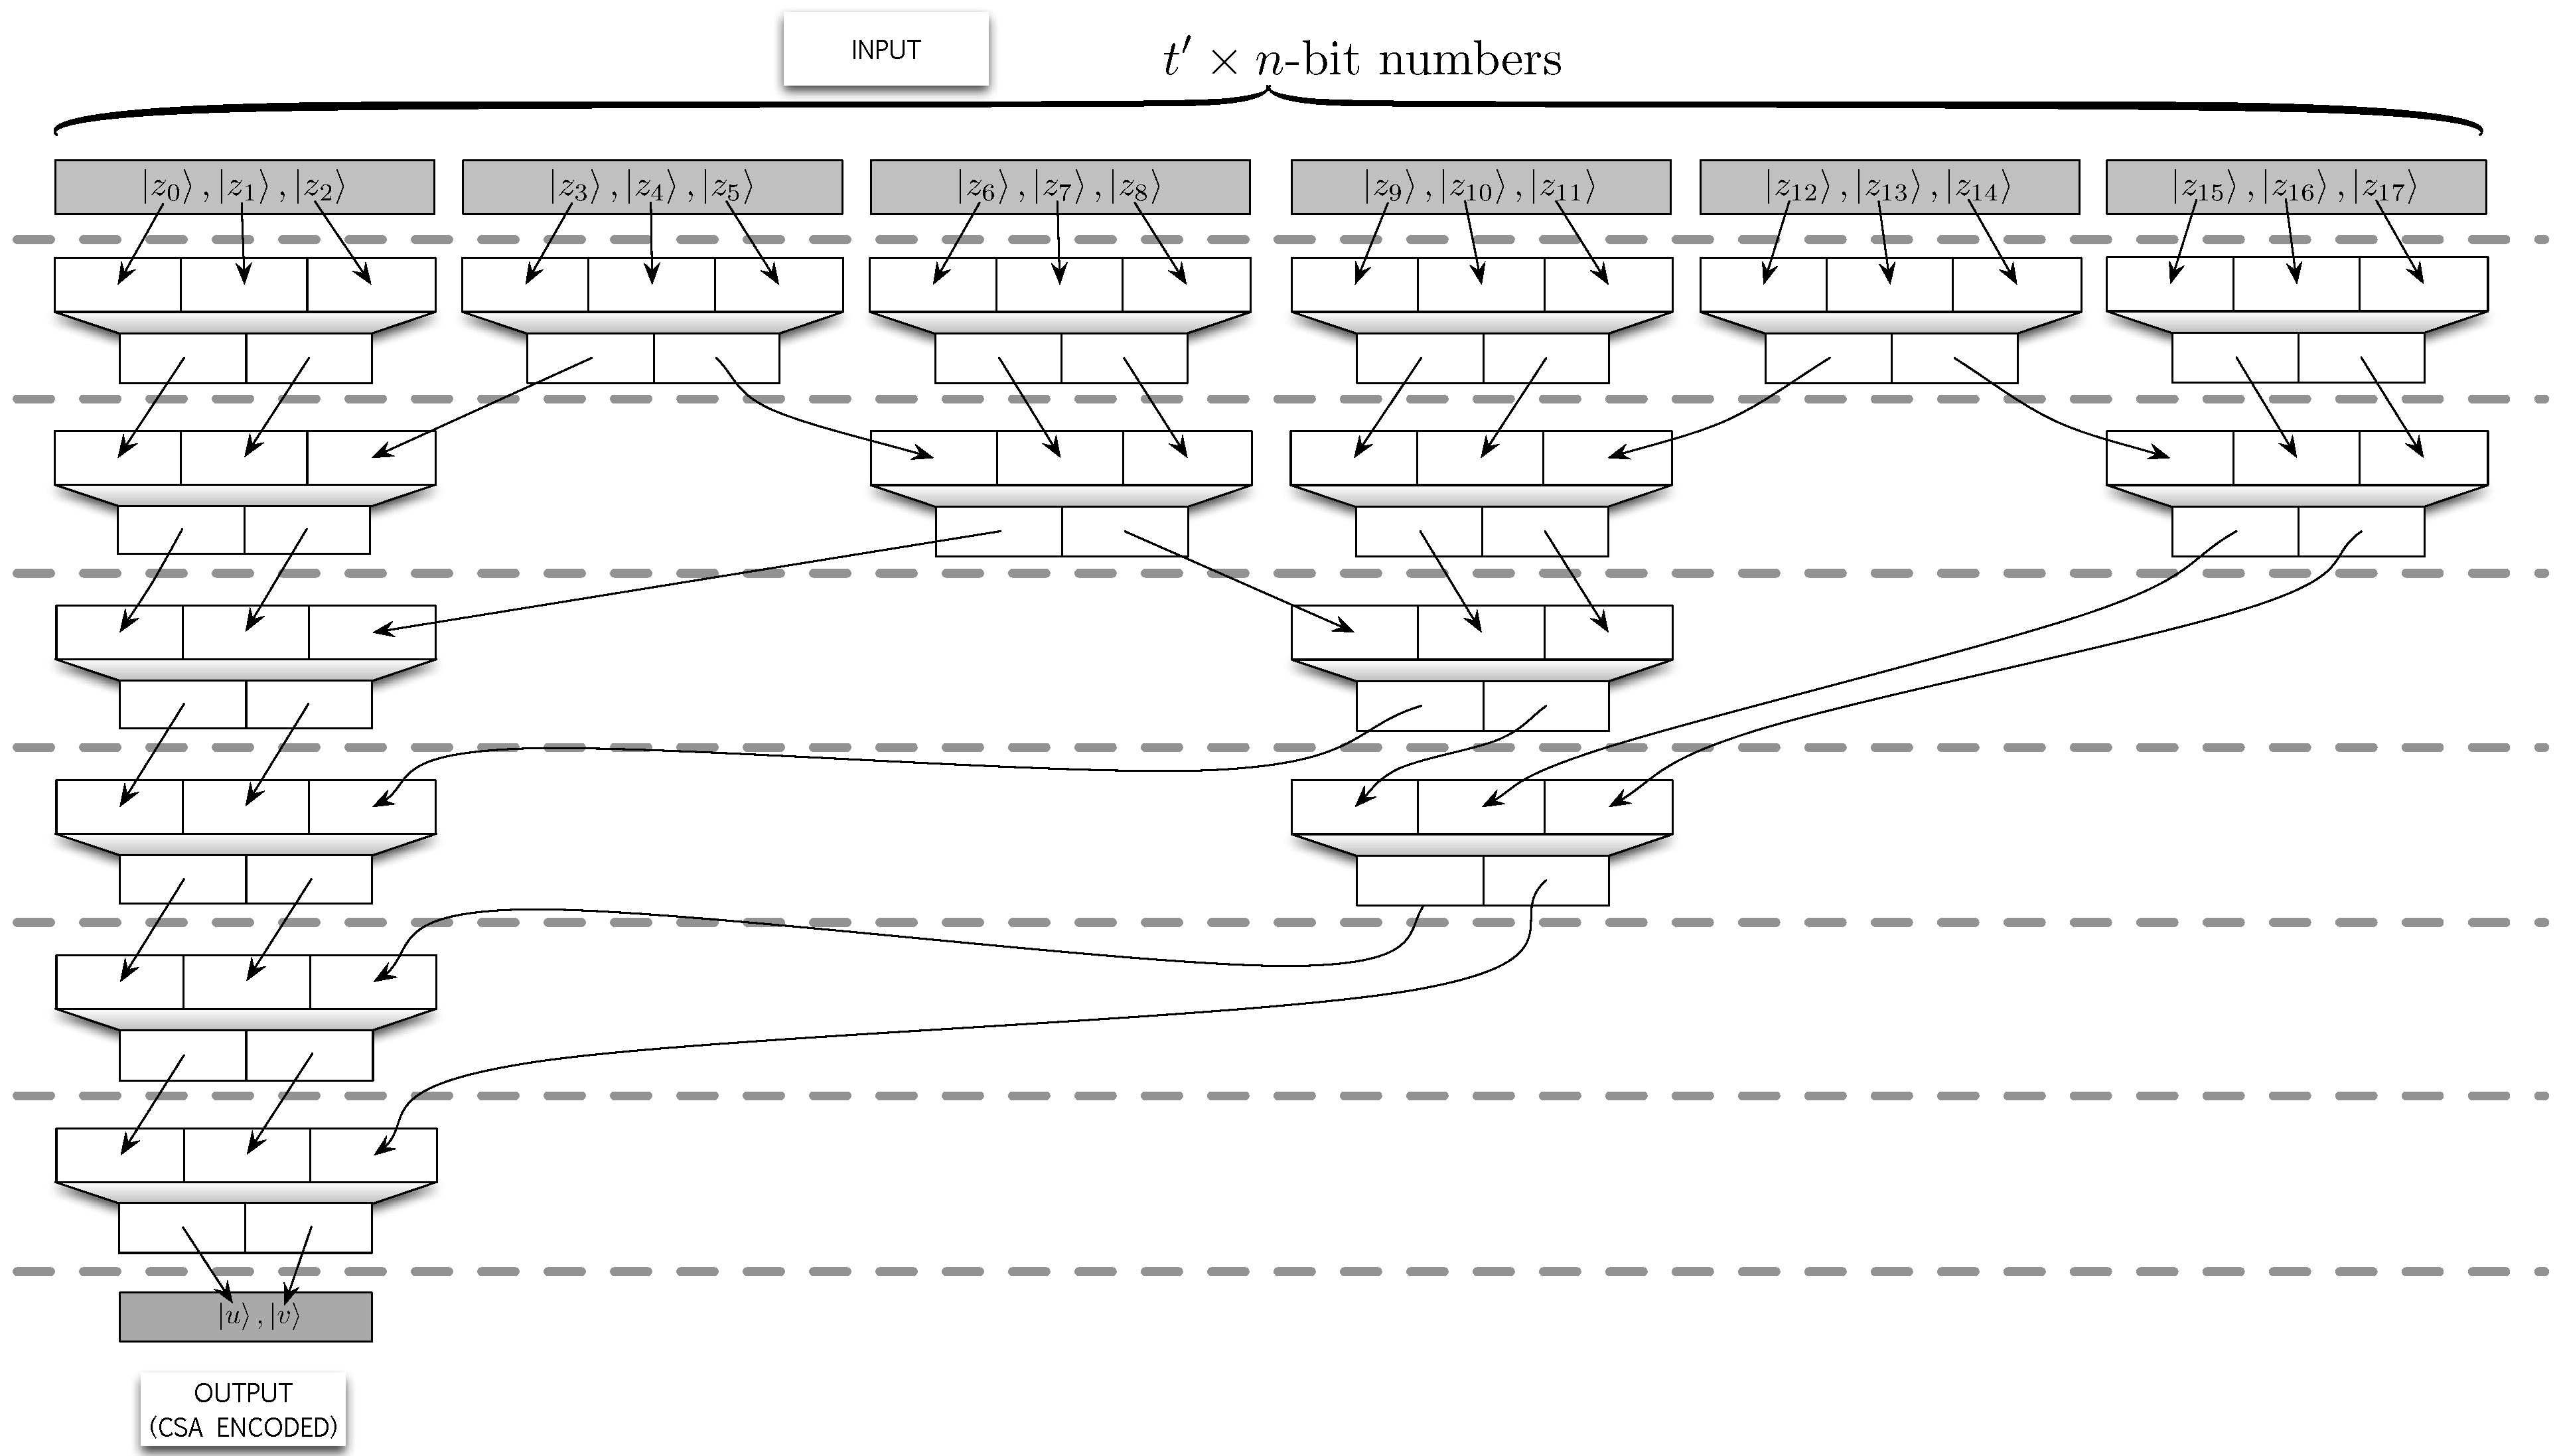
\includegraphics[width=5.5in]{factor-polylog/figures/mod-mult-add.pdf}
}
\caption[Modular multiple addition of quantum integers on a CSA tile
architecture for $t'=18$]
{Modular multiple addition of quantum integers on a CSA tile
architecture for $t'=18$ in a logarithmic-depth tree with height
$(\lceil \log_{\frac{3}{2}}(t'/3) \rceil + 1) = 6$. Arrows represent teleportation
in between modules.}
\label{fig:mod-mult}
\end{figure*}
%

Now we can analyze the circuit resources for multiplying $n$-bit
quantum integers, which requires $(t'-2)$ modular additions, for $t'$ from
Equation \ref{eqn:tprime}.
The circuit width is the sum of the $O(n^3)$ ancillae
needed for partial product creation and the ancillae required for $O(n^2)$
modular additions. Each modular addition has width $O(n)$ and depth $O(1)$
from the previous
section. There are
$\lceil \log_{3/2}(n^2 / 3) \rceil +1 $ timesteps of modular addition. Therefore
the entire modular multiplier circuit has depth $O(\log n)$ and width $O(n^3)$.

\subsection{Modular Multiplier Resources}
\label{subsec:mod-mult-resources}.

The circuit depth of the entire modular multiplier is $O(\log n)$:
%
\begin{equation}
D_{MM} = 1383 \log_2 n + 3930\text{.}
\end{equation}
%
The module depth is $O(\log n)$:
\begin{equation}
\overline{D}_{MM} = 2\log_2 n + 11\text{.}
\end{equation}
%
The circuit size is $O(n^3)$:
%
\begin{eqnarray}
S_{MM} = & (6n + 9)\log_2 n +\\
        & (1152n^3 + 10780n^2 + 17628n + 7082)\text{.}
\end{eqnarray}
%
The module size is $O(n^3)$:
%
\begin{equation}
\overline{S}_{MM} = 15n^3 + 127n^2 + 178n + 50{.}
\end{equation}
%
The circuit width is $O(n^3)$:
%
\begin{equation}
W_{MM} = 66n^3 + 558n^2 + 870n + 290\text{.}
\end{equation}
%
The module width is $O(n^2)$:
%
\begin{equation}
\overline{W}_{MM} = 4n^2 + 28n + 15\text{.}
\end{equation}